\chapter{Background}
The problem space we explore ties together work across a number of different disciplines. In hoping to apply generative methods to vectorized glyphs, we are inspired by previous work in computer vision on non-natural images and draw upon recent developments in generative modeling of line drawings.

\section{Non-natural images}
Natural images are photographs of real-world scenes and objects and to date have been the focus of research in many problems in computer vision, including object recognition, scene segmentation, and image generation.
In contrast, non-natural images are computationally generated, either by hand with a computer design tool or automatically.
Images in this category include graphs, pictograms, virtual scenes, graphic designs, and more.
Algorithmically understanding, summarizing, and synthesizing these images pose unique challenges because of the images' clean and deliberately drawn designs, sometimes multimodal nature, and human-imbued intent. 

Interest in applying computer vision methods to non-natural images is growing.
Much progress has been made towards computationally understanding non-natural images on datasets including XML-encoded scenes~\cite{wu2017neural}, comic strips~\cite{iyyer2016amazing}, and textbook diagrams~\cite{seo2014diagram}.
Recent work by our group has explored the space of infographics, complex diagrams composed of visual and textual elements that deliver a message~\cite{bylinskii2017understanding}.
In this work, we focus specifically on human-crafted font faces.

\subsection{Font faces}
Our computational methods are applied to font faces downloaded from Google Fonts \TODO{cite}. In Figure~\ref{fig:input_fonts}, a sampling of glyphs from the Google Fonts dataset is shown.

As a domain, font glyphs offer certain advantages and pose distinctive challenges. Unlike multimodal infographics and graphic designs, they are drawings essentially composed of simple lines and curves and, as such, can be modeled as sequential drawing commands. \TODO{challenges}

\begin{figure}[]
	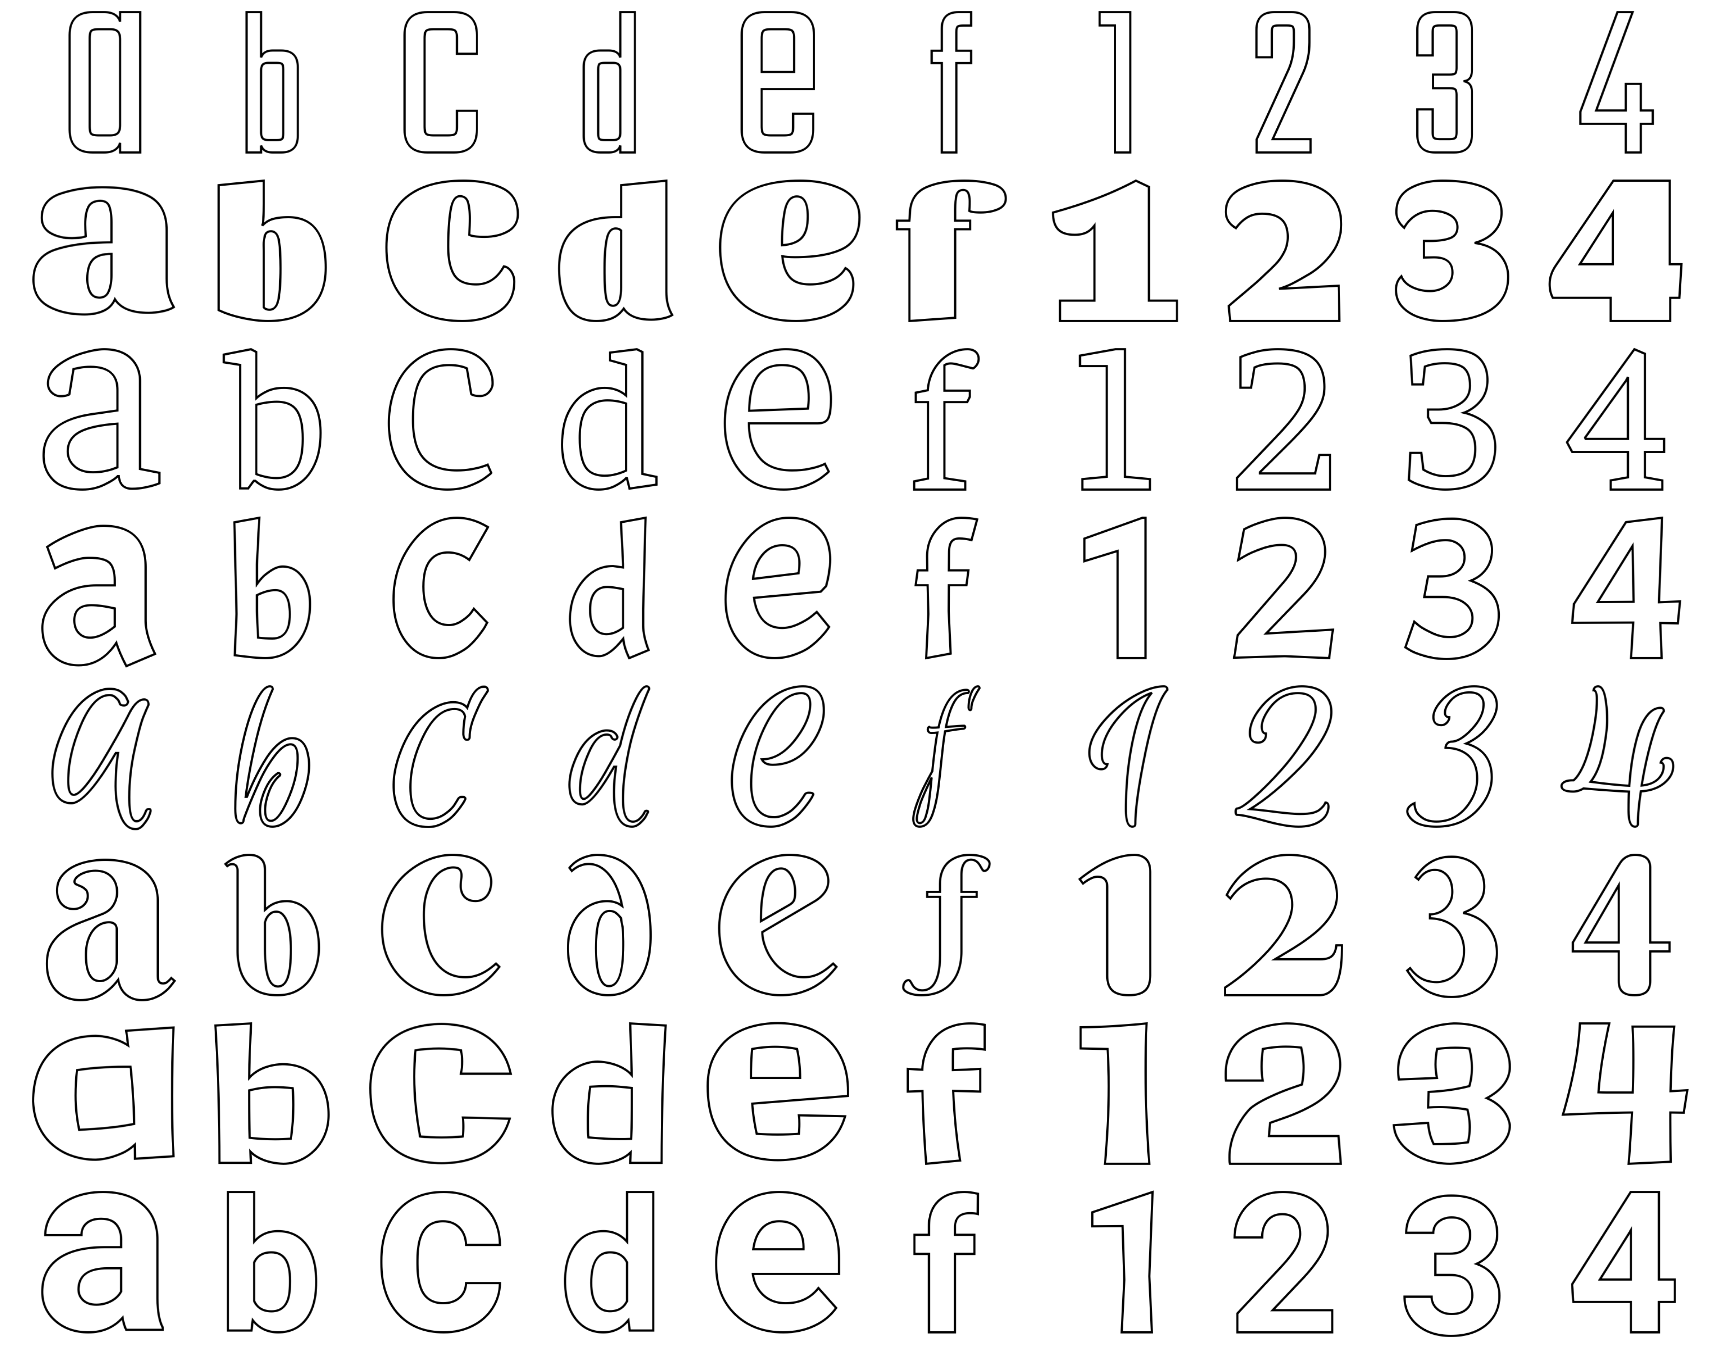
\includegraphics[width=\textwidth]{figures/input_fonts}
    \caption[A sample of the types of font faces used in our fonts dataset]{A sample of the types of font glyphs used in our dataset. Lowercase letters ``a'' through ``f'' are shown, as well as digits 1 through 4. Note the variety of styles represented: the dataset includes serif, sans serif, display, and handwriting style fonts.\label{fig:input_fonts}}
\end{figure}

\subsection{Vector graphics}
In contrast to raster images, which encode color values for each point (or \textit{pixel}) in an image, vector graphics describe a parameterized set of curves and shapes.

Many specifications exist for describing images in vector format, including Scalable Vector Graphics (SVG), Encapsulated PostScript (EPS), and Adobe PDF.

\begin{figure}[t]
    \subcaptionbox{Raster images are defined as two-dimensional arrays of pixel values, while vector graphics define curves and paths mathematically. Thus, when scaled, vector graphics (right) can still be rendered smoothly while raster images (left) degrade in quality.\label{fig:svg-a}}{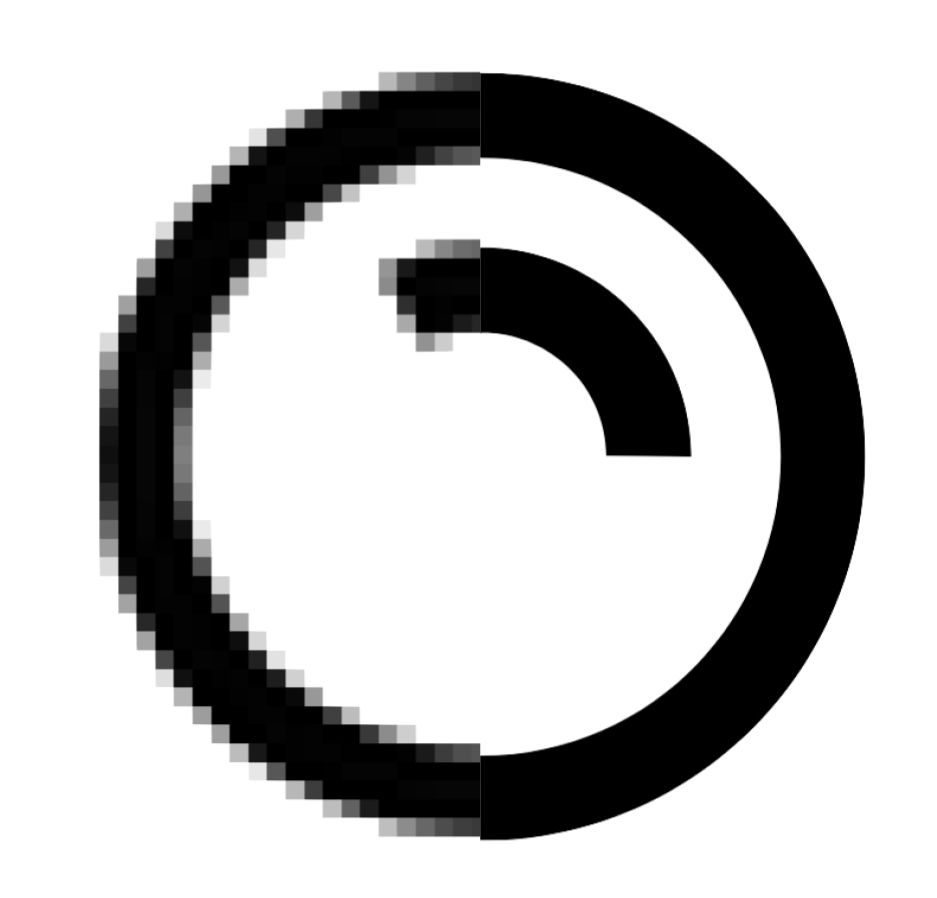
\includegraphics[height=1.85in]{figures/b_vs_vec}} \quad
    \subcaptionbox{SVG is an XML-based markup language that describes geometric elements within a vector image. A single path is used to draw this soap bubble, and colored curves in the image correspond approximately to the highlighted attribute commands that describe them. For example, the command \code{l-0.69-1.32} indicates a line drawn from a starting point to a point 0.69 units to the left and 1.32 units down.\label{fig:svg-b}}{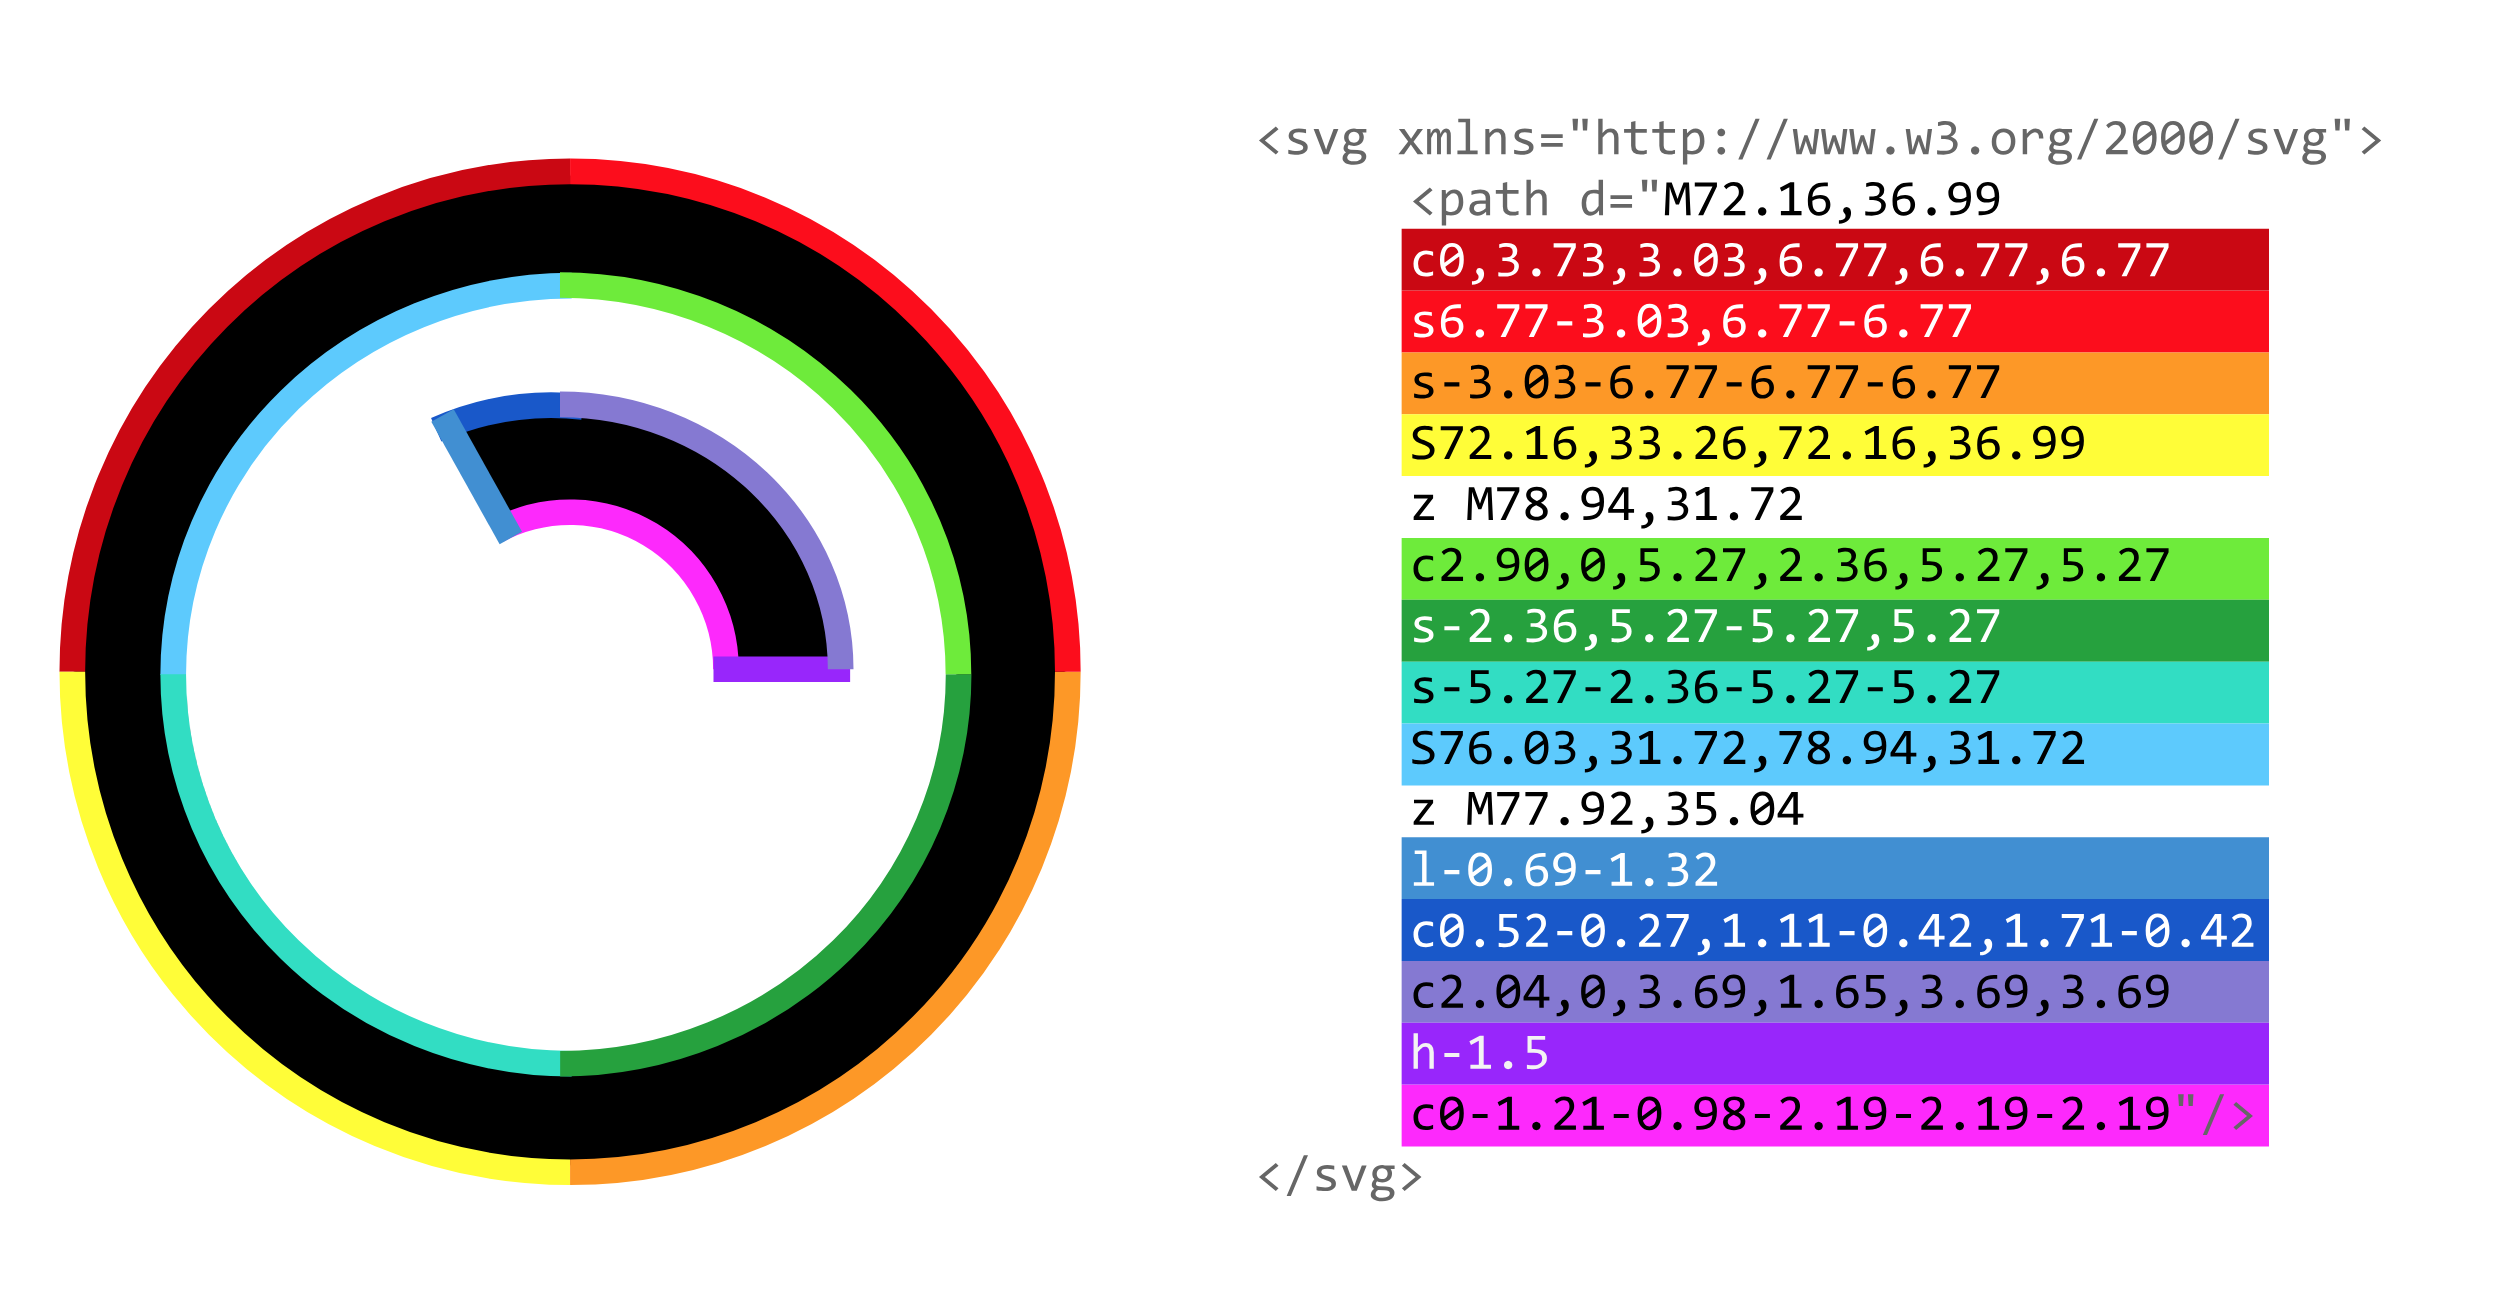
\includegraphics[height=1.85in]{figures/svgs}}
    \caption[An overview of the specification for scalable vector graphics (SVG)]{a visual comparison of raster and vector graphics. Figure~\ref{fig:svg-b} walks through a sample vector graphics path. Image source: \textit{Dog Wash} by Llisole from the Noun Project.\label{fig:svg}}
\end{figure}


\section{Generative modeling}
While discriminative modeling methods in machine learning focus on separating and identifying inputs to produce output labels learned from high-dimensional data such as images, generative algorithms create previously unseen instances of a class based on representative inputs.
They are trained in an unsupervised or semi-supervised manner to model a data distribution $P$, estimating the true data distribution $P_{gt}$ from which samples are drawn.
By drawing probabilistically from $P$, they can then be used to synthesize novel, unseen examples similar to input data.

Two popular neural network-based approaches include generative-adversarial networks (GANs)~\cite{karpathy2016generative} and variational autoencoders (VAEs).
Introduced in~\citeyear{goodfellow2014generative}~\cite{goodfellow2014generative}, GANs pit a generative model $G(z; \theta_g)$ against an adversary $D(x; \theta_g)$ that learns to discriminate samples from the ground truth dataset and the generative model's latent space.
When both models are differentiable functions, backpropagation can be used to train $G$ and $D$ towards convergence in a computationally efficient manner.

\subsection{Variational autoencoders}
Variational autoencoders, introduced in~\cite{kingma2013auto}, explicitly learn an encoder function mapping training examples from the input space $\mathcal{X}$ to a latent space $\mathcal{Z}$ as well as a decoder function mapping from $\mathcal{Z}$ to data points that are in $\mathcal{X}$ but distinct from training inputs $X$.
\TODO{explain more VAE math}

In our work, we specifically build upon the variational autoencoder method in~\cite{ha2017neural}.
\TODO{explain VAE + RNN}

\section{Related work}
\subsection{Image generation}
- DRAW
- SPIRAL
- UToronto handwriting generation
\subsection{Font style}
- Learning a Manifold of Fonts
